\subsection{Identifikation von Maßnahmen}\steffen
Nachdem nun das \emph{SIR}-Modell für die Untersuchung von Pandemien erweitert wurde, werden nun Maßnahmen zur Eindämmung und deren Entsprechung im Netzwerkmodell beschrieben. 

\subsubsection{Lokale Maßnahmen}\steffen
Beginnt eine Krankheit zur Epidemie zu werden, kann man lokal organisatorisch Maßnahmen ergreifen, um sie einzudämmen. Zu diesen zählt die Aufklärung um die Infektionsgefahr sowie die vorübergehende Schließung von öffentlichen Einrichtungen. Letzteres wurde von \cite{Milne2008} mit einem anderen Modell untersucht und für wirksam befunden. Durch die Aufklärung wird die Vorsicht bei zwischenmenschlichen Interaktionen erhöht, was die Infektionswahrscheinlichkeit pro Interaktion senkt. Ähnlich verhält es sich mit der Schließung von öffentlichen Einrichtungen. Hierdurch wird die Anzahl der möglichen Interaktionen von Infizierten und Infizierbaren reduziert, was ebenfalls die Infektionswahrscheinlichkeit reduziert. Im Modell schlagen sich diese Maßnahmen in einer Reduktion der Volumina der inneren Kanten nieder, wie in Abbildung \ref{fig:ssec:actions:local} dargestellt.

\begin{figure}
\begin{center}
\begin{tikzpicture}[->,>=stealth',shorten >=1pt,auto, node distance=3cm]
	\node[state] (S)				{S};
	\node[state] (I)	[right of=S]	{I};
	\node[state] (R)	[right of=I]	{R};
	\path 	(S) edge node {$r\cdot\lambda I$}	(I)
			(I) edge node {$r\cdot\mu I$}		(R);
\end{tikzpicture}
\end{center}
\caption{\emph{SIR}-Modell mit Kantenreduktion um den Faktor $r\in[0,1]$}\label{fig:ssec:actions:local}
\end{figure}


\subsubsection{Impfungen}\steffen
Bei gewissen Klassen von Krankheiten, wie den Viruserkrankungen, lässt sich präventiv ein Schutz vor einer Infektion aufbauen. Im Falle von Viren wäre das die Impfung. Wird ein Individuum vor der eigentlichen Infektion geimpft, immunisiert es sich gegen die Krankheit und ist somit nicht mehr Teil der infizierbaren Subpopulation. Im Modell wird durch das Impfen eine zusätzliche Kante zwischen der $S$ und der $R$ Subpopulation eingefügt. Das Volumen der Kante richtet sich nach Verfügbarkeit und Wirksamkeit der präventiven Maßnahme. Die Verfügbarkeit wird als konstant innerhalb einer Population angesehen. Die Effektivität beschreibt, wieviel Prozent der Empfänger immunisiert werden. Das Volumen der Impfkante ist also unabhängig von der Größe der Infizierbaren. Ein Beispiel dazu ist in Abbildung \ref{fig:ssec:actions:vac} gegeben.
\begin{figure}
\begin{center}
\begin{tikzpicture}[->,>=stealth',shorten >=1pt,auto, node distance=3cm]
	\node[state] (S)				{S};
	\node[state] (I)	[right of=S]	{I};
	\node[state] (R)	[right of=I]	{R};
	\path 	(S) edge node {$\lambda I$}	(I)
			(S) edge [bend left] node {$e\cdot p$}		(R)
			(I) edge node {$\mu I$}		(R);
\end{tikzpicture}
\end{center}
\caption{\emph{SIR}-Modell mit Impfungen. Die Verfügbarkeit der Impfungen wird mit der Konstanten $p\in\mathbb{N}$ und die Effizienz mit dem Faktor $e\in[0,1]$ beschrieben.}\label{fig:ssec:actions:vac}
\end{figure}


\subsubsection{Reisebeschränkungen}\steffen
Während die beiden eben beschriebenen Maßnahmen die Eindämmung einer Krankheit innerhalb der Population als Ziel haben, ist das Ziel der Reisebeschränkung, zu verhindern, dass eine Krankheit in einer bisher gesunden Population ausbricht. Der kanonische Ansatz ist es, kranken Individuen aus anderen Populationen die Einreise zu verwehren. In der Praxis lässt sich dies mit der Sperrung von Grenzen und der Schließung von (Flug-)Häfen realisieren. Stellen die Populationen Länder dar, lässt sich jedoch die vollständige Sperrung von Landwegen zwischen benachbarten Populationen schwer umsetzen. Die Sperrung von (Flug-)Häfen lässt sich als das Entfernen von Reisekanten im Modell darstellen. Bei den Landwegen zwischen benachbarten Populationen ist die Sperrung der Grenze mit einer deutlichen Reduktion der Reisefaktoren gleichzusetzen. 

Der Schutz vor Krankheiten, der durch die Isolation einer Population von den restlichen Populationen entsteht, ist offensichtlich sehr effektiv, setzt man eine reine Mensch-zu-Mensch Übertragung vorraus. Wirtschaftlich kann dieser Schutz eine Population vor große Probleme stellen. Reisekanten, auf denen wirtschaftlich notwendige Güter, wie beispielsweise Nahrungsmittel, transportiert werden, können nicht dauerhaft gesperrt werden. 

\subsubsection{Einreisequarantäne}\steffen
Eine andere Maßnahme, mit der die Einreise kranker Individuen verhindert werden soll, ist die Einrichtung einer Quarantäne bei kontrollierbaren Reisewegen, wie Flugzeugen oder Schiffen. Dabei werden die Einreisenden für eine gewisse Zeit von der restlichen Population isoliert. Erkrankende Individuen werden, im Falle des in dieser Arbeit verwendeten \emph{SEIHFRD}-Modells, hospitalisiert und Individuen, die nicht erkranken, werden in die Population entlassen. Wichtig ist dabei die Dauer der Quarantäne. Da Inkubationszeiten nur statistische Durchschnittwerte sind, kann nie eine Wahrscheinlichkeit von 0 für den Fall erreicht werden, dass ein infiziertes Individuum nicht in die Population entlassen wird. Generell sind lange Quarantänezeiten problematisch in der Umsetzung. Betrachtet man sich beispielsweie das Ebola-Fieber, so wird dessen Inkubationszeit von \cite{Eichner2011} im Schnitt mit $12,7$ Tagen angegeben, bei einer Standardabweichung von $4,3$ Tagen. Um die Wahrscheinlichkeit einer falsch-negativen Infektionsprognose auf $1\%$ zu senken, benötigt man, nach \cite[4]{Eichner2011}, $25$ Tage Quarantäne. Dabei wird voraus gesetzt, dass die Individuen in der Quarantäne sich nicht gegenseitig infizieren können. Je nach Attraktivität der Population, kann es organisatorisch schwer bis unmöglich sein, für alle ankommenden eine $25$-tägige Quarantäne zu verhängen. Die Frage, wie sicher die Quarantäne ist, hängt von den organisatorischen Möglichkeiten der Population, sowie ihrer Einschätzung der Gefährlichkeit der Krankheit ab. 

Im Modell lässt sich eine Quarantäne mit der Einführung zusätzlicher Subpopulationen umsetzen. Für jede reisende Subpopulation, in unserem Modell also $S$ und $E$, wird eine Quarantäne-Subpopulation, $Q_S$ und $Q_E$, eingeführt. Eingehende Kanten kontrollierbarer Reisewege haben dann diese Quarantäne-Subpopulationen als Ziel. Die Quarantäne-Subpopulationen werden mit zugehörigen reisenden Subpopulationen mittels einer inneren Kante unidirektional verbunden, und zwar von der Quarantäne in die Population. Das Volumen der Kanten richtet sich nach der veranschlagten Sicherheit der Quarantäne. Ob es zwischen $Q_S$ und $Q_E$ eine innere Kante gibt, hängt davon ab, ob sich die Individuen in der Quarantäne infizieren können. Weiterhin gibt es eine Kante von $Q_E$ nach $H$, da sichtbar Infizierte direkt hospitalisiert werden. 

\begin{figure}
\begin{center}
\begin{tikzpicture}[->,>=stealth',shorten >=1pt,auto, node distance=3cm]
	\node[state] (S)				{S};
	\node[state] (E) [right =4cm of S]	{E};
	\node (I) [right of=E]	{\dots};
	\node[state] (H) [right of=I]	{H};
	\node[state] (QS)[below of=S] {$Q_S$};
	\node[state] (QE)[below of=E] {$Q_E$};
	\node (X) [below of=QS] {};
	\node (Y) [below of=QE] {};
	\path 	(S)	edge node {$\alpha \cdot (I+E)+ \omega \cdot F$}(E)
			(E)	edge node {}							(I)
			(I)	edge node {}					(H)
			(QS) edge node {$q_S\cdot Q_S$} (S)
			(QS) edge node {$\alpha_Q\cdot Q_E$} (QE)
			(QE) edge node {$q_E\cdot Q_E$} (E)
			(QE) edge[bend right] node {$(1-q_E)\cdot Q_E$}	(H)
			(X) edge node {} (QS)
			(Y) edge node {} (QE)
			;
	
\end{tikzpicture}
\end{center}
\caption{Ausschnitt aus dem SEIHFRD-Modell mit Quarantäne-Subpopulationen $Q_S$ und $Q_E$}\label{fig:ssec:actions:quarantine}
\end{figure}
\subsection{Auswertung der Maßnahmen}\label{ssec:actions:sim}
\subsubsection{Verwendetes Modell}
Im Folgenden werden die soeben beschriebenen Maßnahmen in einem \emph{SEIHFRD}-Modell mit miteinander interagierenden Populationen untersucht. Es werden 5 Populationen in einem einfachen Netzwerk verwendet, das in Abbildung \ref{fig:ssec:sim:pops} dargestellt ist. Die Populationen unterscheiden sich sowohl in ihrem Lebensstandard als auch ihrem Migrationsanteil. Jede Population umfasst $11,5\cdot 10^6$ Individuen, von denen jeweils $4100$ latent infiziert sind. Das \emph{SEIHFRD}-Modell jeder Population ist in Abbildung \ref{fig:ssec:sim:sir} dargestellt. Es wird von einer uniformen Infektionsrate von $2,18$, einer Hospitalisierung von $70\%$ und einer Letalität der Krankheit von $50\%$ ohne und $40\%$ mit Hospitalisierung ausgegangen. Weiterhin finden rituelle Begräbnisse statt, die mit einer Infektionsrate von $0,2$ die Krankheit weiterverbreiten.

\begin{figure}
\begin{center}
\begin{tikzpicture}[-,>=stealth',shorten >=1pt,auto, node distance=4cm]
	\node[state] (A) [text width=2cm,align=center] {\textbf{A}\\$L_A=2$\\$M_A=0,1$};
	\node[state] (B) [text width=2cm,align=center,right of=A]	{\textbf{B}\\$L_B=1$\\$M_B=0,3$};
	\node[state] (C) [text width=2cm,align=center,right of=B]	{\textbf{C}\\$L_C=1$\\$M_C=0,2$};
	\node[state] (D) [text width=2cm,align=center,above of=B]	{\textbf{D}\\$L_D=0,5$\\$M_D=0,2$};
	\node[state] (E) [text width=2cm,align=center,below of=B]	{\textbf{E}\\$L_E=2$\\$M_E=0,2$};
	\path	(A) edge node {} (B)
			(A) edge node {} (E)
			(B) edge node {} (C)
			(B) edge node {} (D)
			(B) edge node {} (E)
			(C) edge node {} (D);
\end{tikzpicture}
\end{center}
\caption{Populationsnetzwerk für die Simulation. Ungerichtete Kanten repräsentieren bidirektionale Wege}\label{fig:ssec:sim:pops}
\end{figure}


\begin{figure}
\begin{center}
\begin{tikzpicture}[->,>=stealth',shorten >=1pt,auto, node distance=3cm]
	\node[state] (S)				{S};
	\node[state] (E) [right =4.5cm of S]	{E};
	\node[state] (I) [right =3.5cm of E]	{I};
	\node[state] (H) [right of=I]	{H};
	\node[state] (F)[above of=I]	{F};
	\node[state] (D)[right of=F]	{D};
	\node[state] (R)[below of=H]	{R};
	\node (QS)[below of=S] {};
	\node (QE)[below of=E] {};
	\node (X) [above of=S] {};
	\node (Y) [above of=E] {};
	\path 	(S)	edge node {$2,18 \cdot (I+E)+ 0,2 \cdot F$}(E)
			(E)	edge node {$(1-M_X) \cdot E$}							(I)
			(I)	edge node {$0,15 \cdot I$}						(F)
			(I)	edge node {$0,7\cdot I$}					(H)
			(I)	edge [bend right] node {$0,15 \cdot I$}					(R)
			(F)	edge node {$F $}						(D)
			(H)	edge node {$0,4\cdot H$}					(D)
			(H) edge node {$0,6 \cdot H $}				(R)
			(QS) edge node {$T^{*,X}$} (S)
			(QE) edge node {$T^{*,X}$} (E)
			(S) edge node {$T^{X,*}$} (X)
			(E) edge node {$T^{X,*}$} (Y)
			;
	
\end{tikzpicture}
\end{center}
\caption{SEIHFRD-Modell für die Auswertung der Maßnahmen mit $X \in \lbrace A,B,C,D,E\rbrace$ und $M_X$ dem Migrationsanteil von $X$}\label{fig:ssec:sim:sir}
\end{figure}
\ellen
Nachdem die Simulation durchgeführt wurde, wurden die Ergebnisse mit Hilfe von Excel ausgewertet. Dabei zeigt sich, dass die größten Veränderungen in der Population A auftreten.\\
\begin{figure}
 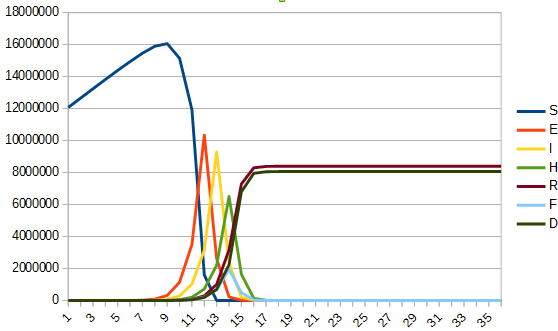
\includegraphics[width=1\textwidth]{massnahmen/A0}
\caption{Population A ohne Einflussnahme}
\label{fig:ssec:actions:A0}
\end{figure}
 Bei Abbildung \ref{fig:ssec:actions:A0} handelt es sich um den Krankheitsverlauf, innerhalb der Population A, ohne Einflussnahme. Dabei kann man sehen, dass die Anzahl der gesunden Individuen innerhalb der Population zunächst ansteigt. Dies ist auf die Migration zurückzuführen. Etwa die Hälfte der Bevölkerung überlebt die Epidemie und bildet eine Immunität aus (51\%).\\
 \begin{figure}
 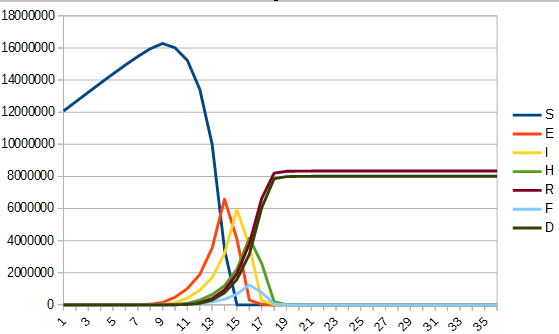
\includegraphics[width=1\textwidth]{massnahmen/A1}
\caption{Population A mit erhöhter Hygiene}
\label{fig:ssec:actions:A1}
\end{figure}
Durch die erhöhte Hygiene und die daraus resultierende geringere Ansteckungsrate, kommt es nur zu geringen Unterschieden im Krankheitsverlauf. Wie zu erwarten steigt die Anzahl der Infizierten langsamer an als vorher. Zusätzlich befinden sich am Ende weniger Menschen in dieser Population. Ohne Maßnahmen gibt es 16.466.684 Immune und Tote in A, während es bei erhöhter Hygiene lediglich 16.351.824 sind. Dies könnte darauf zurückgeführt werden, dass durch die verlangsamte Krankheitsausbreitung die Zeit für Migration verlängert wird. Die Überlebensrate steigt leicht auf 51,03\%. Siehe dazu die Abbildung \ref{fig:ssec:actions:A1}\\
 \begin{figure}
 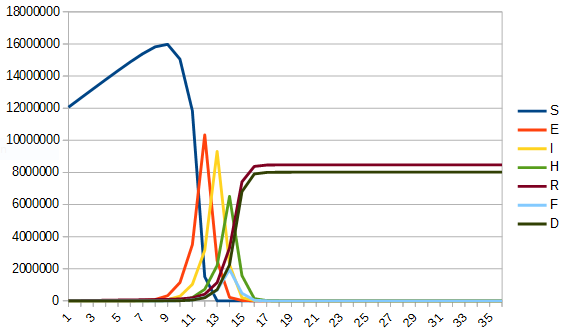
\includegraphics[width=1\textwidth]{massnahmen/A2}
\caption{Population A mit Impfen}
\label{fig:ssec:actions:A2}
\end{figure}
  Durch das Impfen steigt die Immunisierungsrate an. Dadurch steigt die Überlebensrate auf 51,39\%. Siehe dazu Abbildung \ref{fig:ssec:actions:A2}.\\
  \begin{figure}
 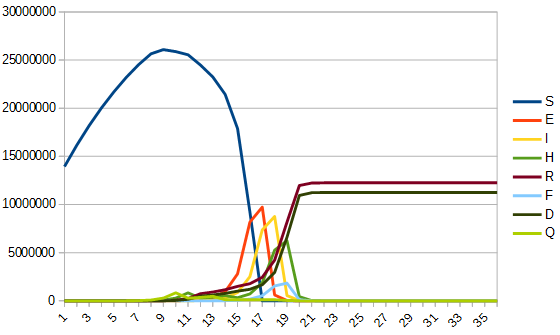
\includegraphics[width=1\textwidth]{massnahmen/A3}
\caption{Population A mit Quarantäne}
\label{fig:ssec:actions:A3}
\end{figure}
  Durch die Quarantäne steigt die Überlebensrate sogar stärker an als zuvor (auf 52,14\%). Dies kann jedoch auch daran liegen, dass sich die Zuwanderung signifikant verändert hat. Wodurch dies ausgelöst wird, ist durch die vorliegenden Daten nicht ersichtlich, jedoch befinden sich am Ende der Simulation 23.508.184 Tote und Immune in der Population A. Siehe dazu Abbildung \ref{fig:ssec:actions:A3}.\\
 \begin{figure}
 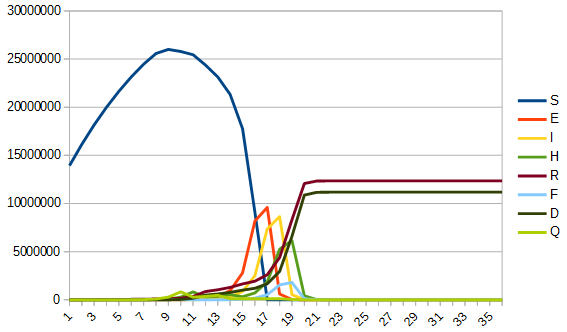
\includegraphics[width=1\textwidth]{massnahmen/A4}
\caption{Population A mit Impfen und Quarantäne}
\label{fig:ssec:actions:A4}
\end{figure}
  Wie zu erwarten war, steigt die Überlebensrate weiter an, wenn zwei Maßnahmen kombiniert werden.\\
  Zusätzlich bleibt die Gesamtpopulation erhöht, sogar leicht höher als bei der Quarantäne alleine. Es befinden sich nun 23.542.177 Immune und Tote innerhalb der Population. Siehe dazu Abbildung \ref{fig:ssec:actions:A4}\\
   Bei den weiteren Populationen ist der Einfluss der Maßnahmen sehr gering. Dies könnte unter anderem daran liegen, dass der auswandernde Anteil an der Population A der geringste ist. Somit sind die anderen Populationen von einer größeren Abwanderung betroffen.\\
   In den anderen Populationen liegt die Überlebensrate immer bei etwa 51\%. Es gibt jedoch Populationen, bei denen die Einflussname zu geringeren Überlebensquoten führt. Dies liegt jedoch, wie bereits erwähnt eher an den Migrationsbewegungen als an einer wirklichen Verschlechterung der Situation.\\
   Durch die Auswertung wurde ersichtlich, dass das Modell die Realität noch nicht ausreichend abbildet. Das hier vorgestellte und untersuchte Modell kann nahezu beliebig weitergeführt werden. Beispielsweise können weitere Maßnahmen implementiert werden, dazu gehören Schulschließungen oder Einreisestopps.\\
   Um dieser Komplexität gerecht zu werden, kann die Simulation für Projektwochen eingesetzt werden. Es handelt sich dabei offensichtlich um eine Kombination aus Mathematik und Informatik. Hinzu kommen jedoch auch Schnittmengen mit den Fächern Deutsch -- durch das einüben von Lesekompetenz und Formulierungen über Zusammenhänge --, Geschichte -- durch die Betrachtung früherer Epidemien --, Sozialkunde -- durch die Urteilsbildung bezüglich der durchführbaren Maßnahmen -- und weitere andere.\\
   Bei der Umsetzung für diese Arbeit stand jedoch keine Projektwoche zur Verfügung, weshalb lediglich das grundlegende Modell simuliert und ausgewertet wurde.
